% Usage: knitr slide


\chapter{\R}\alabel{chap:R}
\section{Background}
Computer code shown throughout these notes is \R~\cite{R}.  \R\ is free
and is the 
most widely used statistical software in the world.  It has the best graphics,
statistical modeling, nonparametric methods, survival analysis,
clinical trials methods, and data manipulation capabilities.  \R\ has
the most comprehensive genomics analysis packages and has advanced
capabilities for reproducible analysis and reporting.  \R\ also has an
excellent graphical front-end \Co{RStudio} (\href{https://www.rstudio.com/}{rstudio.org}) that
has the identical look and feel on all operating systems and via a web
browser.  Part of
\R's appeal is the thousands of add-on packages available (at
\url{http://cran.r-project.org/web/packages}), which 
exist because it is easy to add to \R.  Many of the add-on packages
are specialty packages for biomedical research including packages for
such widely diverse areas as
\bi
\item interfacing \R\ to \Co{REDCap} (2 packages)
\item interactive design of adaptive clinical trials
\item analyzing accelerometer data
\item flow cytometry
\item genomics
\item analyzing ICD9 codes and computing comorbidity indexes
\item downloading all annotated NHANES datasets
\item interfacing to \href{https://clinicaltrials.gov/}{clinicaltrials.gov}
\item detecting whether a dataset contains personal identifiers of
  human subjects
\item analysis of early phase cardiovascular drug safety studies
\ei
The main \R\ web site is \href{https://www.r-project.org/}{www.r-project.org}.

\section{Learning \R}
Start with \emph{R Tutorials} at \url{http://www.r-bloggers.com/how-to-learn-r-2} and \emph{R Programming Tutorials} from Mike Marin at
\url{https://www.youtube.com/user/marinstatlectures}.  Or look at
\url{swirlstats.com} for an interactive way to learn \R. Those
who have used SPSS or SAS before will profit from \emph{\R\ for SAS
  and SPSS Users} by Robert Muenchen.  A current list of \R\ books on
\href{https://www.amazon.com/}{amazon.com} may be found at \url{http://amzn.to/15URiF6}.
\url{https://stats.idre.ucla.edu/r/} and
\url{http://www.introductoryr.co.uk/R_Resources_for_Beginners.html}
are useful web sites. See also \emph{\R\ in Action, second ed.} by Robert 
Kabacoff.  The online open source book on statistical modeling by Legler and Roback at
\url{https://bookdown.org/roback/bookdown-bysh} contains a lot of \R\ code.
\url{http://stackoverflow.com/tags/r} is the best place for asking
questions about the language and for learning from answers to past questions
asked (see also the \Co{R-help} email list).

Three of the best ways to learn how to analyze data in \R\ quickly are
\be
\item Avoid importing and manipulating data, instead using the \R\
  \co{load} function to load datasets that are already annotated and
  analysis-ready (see Section~\ref{sec:r-import} for information about
  importing your own datasets)
\item Use example \R\ scripts as analysis templates
\item Use \co{RStudio} (\href{https://www.rstudio.com/}{rstudio.org}) to run \R
\ee
On the first approach, the \R\ \co{Hmisc} packages's \co{getHdata}
function finds datasets on the Vanderbilt Biostatistics \co{DataSets}
wiki, downloads them, and \co{load()}s them in your \R\ session.
These notes use only datasets available via this mechanism.  These
datasets are fully annotated with variable labels and units of
measurements for many of the continuous variables.
Concerning analysis scripts, Vanderbilt Biostatistics has collected
template analysis scripts on
\url{https://github.com/harrelfe/rscripts}\footnote{\co{github} has
  outstanding version control and issue reporting/tracking.  It
  greatly facilitates the contribution of new scripts by users, which
  are most welcomed.  Contact \texttt{f.harrell@vanderbilt} if you
  have scripts to contribute or suggestions for existing scripts.} and
the \R\ \co{Hmisc} package has a function \co{getRs} to download these
scripts and to automatically populate an 
\co{RStudio} script editor window with the script.
Many of the scripts are in RMarkdown format for use with the \R\
\co{knitr} package to allow mixing of text and \R\ code to make
reproducible reports.  \co{knitr} is described in 
Section~\ref{sec:repro-software}.

The RMarkdown scripts accessed through \co{getRs} use a template that makes the
result part of 
a reproducible research process by documenting the versions of \R\ and
attached packages at the end of the report.  Some of the scripts make use of the
\co{knitrSet} function in the \co{Hmisc} package. When running
Rmarkdown, call \co{knitrSet(lang='markdown')}.  \co{knitrSet} gets
rid of \verb|##| at 
the start of R output lines, and makes it easy to specify things like
figure sizes in knitr chunk headers. It also causes annoying messages
such as those generated from attaching \R\ packages to be put in a
separate file \co{messages.txt} rather than in the report.

\section{Setting up \R}
Before running examples in these notes and \R\ markdown example
scripts, you need to do the following:
\be
\item Make sure your operating system is up to date enough to run the
  most current version of \R\ at \href{https://www.r-project.org/}{www.r-project.org}.  For Mac you
  must have OS X Maverick or later.
\item Install \R\ from \href{https://www.r-project.org/}{www.r-project.org} or upgrade your
  installation of \R\ to the latest version.
\item Install \co{RStudio} from \href{https://www.rstudio.com/}{rstudio.org} or update your
  \co{RStudio} to the latest version.
%\item Download and store the \co{.Rprofile} file using instructions at
%  \url{http://biostat.mc.vanderbilt.edu/RConfiguration}.  This defines
%  \co{getRs}, \co{knitrSet}, and several other useful functions.
%\item If you are running Windows or Mac OSX follow the
%  instructions at the same web page for installing
%  \co{wget}\footnote{\co{github} only allows files to be accessed
%    using an \co{https} protocol, and \R\ by default does not allow
%    accessing web pages by \co{https}.  \R's \co{download.file} and
%    other functions can access \co{https} pages using the
%    \co{method='wget'} option, which is how \co{getRs} works.}
\item Run \co{RStudio} and get it to install the packages that allow
  \co{Rmarkdown} to run, by clicking on \co{File ... New File ... R
    Markdown}.  Make sure that the \co{knitr} package is installed.
\item Have \co{RStudio} install the \co{Hmisc} and \co{rms} packages
  (which will make \co{RStudio} install several other packages).  For
  packages you had installed previously, make sure you update them to
  have the latest versions.
\item Configure \co{RStudio} \co{Tools ... Global Options} to match
  the images below
  
\centerline{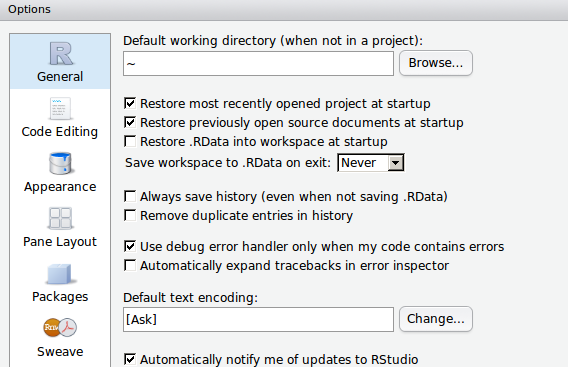
\includegraphics[width=.5\textwidth]{rstudioOptions.png}}

\bigskip

\centerline{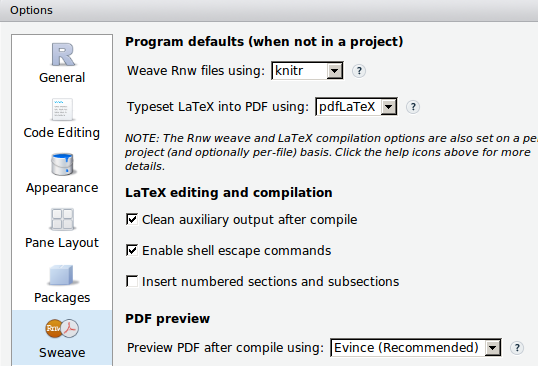
\includegraphics[width=.5\textwidth]{rstudioSweave.png}}
\ee
Here are some examples of how \co{getRs} is used once you
load the \co{Hmisc} package using a menu or by typing
\co{require(Hmisc)} or \co{library(Hmisc)} in the console.
\begin{Schunk}
\begin{Sinput}
require(Hmisc)      # do this once per session (or library(Hmisc))
options(url.method='libcurl')    # sometimes needed if using Windows
getRs()             # list available scripts
getRs(browse='browser')  # open scripts contents in your web browser
scripts <- getRs()  # store directory of scripts in an object that can easily
                    # be viewed on demand in RStudio (right upper pane)
getRs('introda.r')  # download introda.r and open in script editor
getRs(cats=TRUE)    # list available major and minor categories
categories <- getRs(cats=TRUE)  # store results in a list for later viewing
getRs(cats='reg')   # list all scripts in a major category containing 'reg'
getRs('importREDCap.r', put='source')   # source() to define a function
\end{Sinput}
\end{Schunk}
You can also point your browser to
\url{https://github.com/harrelfe/rscripts/blob/master/contents.md} to
see the available scripts and categories, and to be able to click on
links to see \co{html} report output.

To get started using \R\ in \co{RStudio} to create reproducible
annotated reports, finish the above configuration instructions and
type the following in the \co{RStudio} console:
\co{getRs('descriptives.Rmd')}.  The above the script editor window
click on \co{Knit HTML}.

\section{Using R Markdown}
See \url{http://kbroman.org/knitr_knutshell/pages/Rmarkdown.html} and
print the \co{R Markdown} cheat sheet from
\url{http://www.rstudio.com/resources/cheatsheets}.

To make the code listing pretty, put this chunk at the top of your
report.  \co{echo=FALSE} suppresses this setup chunk from printing in
the report.
\begin{verbatim}
```{r setup,echo=FALSE}
require(Hmisc)
knitrSet('myreport', lang='markdown')
```
\end{verbatim}
The argument \co{'myreport'} is replaced with a string to use as a
prefix to all the graphics file names, making each report in your
working directory use graphics file names that do not collide with
each other.  For example if your report is called
\co{acidity\_analysis.Rmd} you might specify
\co{knitrSet('acidity\_analysis.Rmd', lang='markdown')}.  There are
many other options to \co{knitrSet}.  A commonly used one is
\co{width=n} to specify a line width for printing code of \co{n} letters.  The
default is 61.  You can also specify \co{echo,results}, and other
options.  Type \co{?knitrSet} for help.

The \R\ \co{knitr} package is used to run the markdown report and
insert graphics and text output into the report at appropriate slots.
It is best to specify a name for each chunk, and you must use unique
names.  Each \R\ code chunk must begin exactly
with \verb|```{r ...}| and the chunk name is the first set of
characters that appear after the space after \verb|r|.  Here are some
example chunk headers.  Chunk names must not contain a space.
\begin{verbatim}
```{r descriptives}
```{r anova}
```{r anova-y1}
```{r anova_y1}
```{r acidity_plot}
```{r plot_residuals,top=1}
```{r plot_residuals,mfrow=c(2,2),left=1,top=1,rt=1,bot=1}
```{r plot-residuals,w=5,h=4}
\end{verbatim}
Chunk options that were used above are:
\begin{center}\begin{tabular}{ll}
  Options & Description \\ \hline
  \co{top=1} & Leave an extra line of space at top of graph for title \\
  \co{mfrow=c(2,2)} & Use base graphics and put the next 4 plots into a\\
                    & single figure with 2 rows, 2 columns\\
  \co{left=1,rt=1,bot=1} & Leave one extra line for margin for left,
                           right, bottom of figure\\
  \co{w=5,h=4} & Make the figure larger than the default that
                 \co{knitrSet} uses\\
               & (4 inch width by 3 inch height) \\ \hline
  \end{tabular}\end{center}

Always having a chunk name also allows easy navigation of chunks by
clicking to the right of the green \co{C} at the bottom of your
script.  This will show the names of all chunks and you can click on
one to go there.

\section{Debugging \R\ Code}
When using \co{RStudio} and \co{knitr} as with \co{RMarkdown}, it is
best to debug your commands a piece at a time.  The fastest way to do
this is to go to some line inside your first chunk and click the green
\co{C} just above and to the right of your script.  Click on \co{Run
  Current Chunk} then on \co{Run Next Chunk}.  Shortcut keys for these
are \co{Ctrl+Alt+C} and \co{Ctrl+Alt+N} (\co{Command+Option+C} and \co{Command+Option+N} for Mac).  You can also click on a
single line of code and run it by clicking on \co{Run}.

Whenever you get a strange execution error it is sometimes helpful to
show the history of all the function calls leading to that error.
This is done by typing \co{traceback()} at the command prompt.

\section{Importing Other Datasets}\alabel{sec:r-import}
Most of the work of getting some data sources ready for analysis involves
reshaping datasets from wide to tall and thin, recoding variables,
and merging multiple datasets.  \R\ has first-class capabilities for
all of these tasks but this part of \R\ is harder to learn, partly
because there are so many ways to accomplish these tasks in \R.
Getting good variable names, variable labels, and value labels, can
also be tedious but is highly worth the time investment.

\subsection{Stata and SPSS}
If you have Stata or SPSS files that are
already shaped correctly and have variable labels and value
labels, the \R\ \co{Hmisc} package's \co{stata.get} and
\co{spss.get} functions will produce fully annotated
ready-to-analyze \R\ data frames.


\subsection{REDCap}
\co{REDCap} exports data to \R, and Biostatistics has an \R\ function
to make the import process much easier.  Here is an example showing
how to fetch and use the function.  In this example, the user did not
provide the name of the file to import but rather let the function
find the last created REDCap export files in the current working directory.
\begin{Schunk}
\begin{Sinput}
require(Hmisc)
getRs('importREDCap.r', put='source')  # source() code to define function
mydata <- importREDCap()  # by default operates on last downloaded export
Save(mydata)   # Hmisc function to create mydata.rda in compressed format
\end{Sinput}
\end{Schunk}

Advanced users can hook into
\co{REDCap} dynamically with \R\ to avoid the need to export/import.

\subsection{Spreadsheets}
If you have a properly
formatted \co{csv} file (e.g., exported from a spreadsheet), the
\co{Hmisc} \co{csv.get} function will read it, facilitate handling
of date variables, convert column names to legal \R\ names, and
save the original column names as variable labels.

Here is an example of importing a \co{csv} file into \R.  First of all
make sure your spreadsheet is a ``spreadsheet from heaven'' and not a
``spreadsheet from hell'' by reading
\url{http://biostat.mc.vanderbilt.edu/DataTransmissionProcedures}.
Then use your spreadsheet software to export a single worksheet to
create a \co{csv} file.  Small \co{csv} files may be pasted into your
\R\ script as is done in the following example, but in most cases you
will call \co{csv.get} with an external file name as the first
argument.

\begin{Schunk}
\begin{Sinput}
# What is between data <- .. and ') is exactly like an external .csv file
data <- textConnection('
Age in Years,sex,race,visit date,m/s
23,m,w,10/21/2014,1.1
14,f,b,10/22/2014,1.3
,f,w,10/15/2014,1.7
')
require(Hmisc)
d <- csv.get(data, lowernames=TRUE, datevars='visit.date',
             dateformat='%m/%d/%Y')
close(data)
# lowernames=TRUE: convert variable names to lower case
# Omit dateformat if dates are in YYYY-MM-DD format
contents(d)
\end{Sinput}
\begin{Soutput}

Data frame:d	3 observations and 5 variables    Maximum # NAs:1


                   Labels Levels   Class Storage NAs
age.in.years Age in Years        integer integer   1
sex                   sex      2         integer   0
race                 race      2         integer   0
visit.date     visit date           Date  double   0
m.s                   m/s        numeric  double   0

+--------+------+
|Variable|Levels|
+--------+------+
|  sex   |  f,m |
+--------+------+
|  race  |  b,w |
+--------+------+
\end{Soutput}
\begin{Sinput}
d
\end{Sinput}
\begin{Soutput}
  age.in.years sex race visit.date m.s
1           23   m    w 2014-10-21 1.1
2           14   f    b 2014-10-22 1.3
3           NA   f    w 2014-10-15 1.7
\end{Soutput}
\end{Schunk}
In the \co{contents} output above you can see that the original column
names have been placed in the variable labels, and the new names have
periods in place of blanks or a slash, since these characters are
illegal in \R\ names.

You can have as the first argument to \co{csv.get} not only a file
name but a URL to a file on the web.  You can also specify delimiters
other than commas.

Also see the excellent tutorial on importing from Excel found at \url{http://www.r-bloggers.com/r-tutorial-on-reading-and-importing-excel-files-into-r}.

The \co{Hmisc} \co{upData} function may be used to rename variables
and provide variable and value labels and units of measurement.
Here is another example where there is a \co{junk} variable to
delete after importing, and a categorical variable is coded as
integers and need to have value labels defined after
importing.  We show how \co{csv.get} automatically renamed one illegal
(to \R) variable name, how to redefine a variable label, and how to
define the value labels.  Suppose that file \co{test.csv} exists in
our project directory and has the following contents.
{\small\begin{verbatim}
age,sys bp,sex,junk,state
23,140,male,1,1
42,131,female,2,1
45,127,female,3,2
37,141,male,4,2
\end{verbatim}}
Now import and modify the file.
\begin{Schunk}
\begin{Sinput}
require(Hmisc)
d <- csv.get('test.csv')
names(d)   # show names after modification by csv.get
\end{Sinput}
\begin{Soutput}
[1] "age"    "sys.bp" "sex"    "junk"   "state" 
\end{Soutput}
\begin{Sinput}
contents(d)  # show labels created by csv.get
\end{Sinput}
\begin{Soutput}

Data frame:d	4 observations and 5 variables    Maximum # NAs:0


       Labels Levels   Class Storage
age       age        integer integer
sys.bp sys bp        integer integer
sex       sex      2         integer
junk     junk        integer integer
state   state        integer integer

+--------+-----------+
|Variable|Levels     |
+--------+-----------+
|   sex  |female,male|
+--------+-----------+
\end{Soutput}
\begin{Sinput}
d <- upData(d,
            state=factor(state, 1:2, c('Alabama','Alaska')),
            rename=c(sys.bp='sbp'),
            labels=c(age = 'Age',
                     sbp = 'Systolic Blood Pressure'),
            drop='junk',   # for > 1: drop=c('junk1','junk2',...)
   units=c(sbp='mmHg'))
\end{Sinput}
\begin{Soutput}
Input object size:	 3848 bytes;	 5 variables	 4 observations
Renamed variable	 sys.bp 	to sbp 
Modified variable	state
Dropped variable	junk
New object size:	3456 bytes;	4 variables	4 observations
\end{Soutput}
\begin{Sinput}
contents(d)
\end{Sinput}
\begin{Soutput}

Data frame:d	4 observations and 4 variables    Maximum # NAs:0


                       Labels Units Levels   Class Storage
age                       Age              integer integer
sbp   Systolic Blood Pressure  mmHg        integer integer
sex                       sex            2         integer
state                                    2         integer

+--------+--------------+
|Variable|Levels        |
+--------+--------------+
|  sex   |female,male   |
+--------+--------------+
|  state |Alabama,Alaska|
+--------+--------------+
\end{Soutput}
\begin{Sinput}
describe(d)
\end{Sinput}
\begin{Soutput}
d 

 4  Variables      4  Observations
---------------------------------------------------------------------------
age : Age 
       n  missing distinct     Info     Mean      Gmd 
       4        0        4        1    36.75    11.83 
                              
Value        23   37   42   45
Frequency     1    1    1    1
Proportion 0.25 0.25 0.25 0.25
---------------------------------------------------------------------------
sbp : Systolic Blood Pressure [mmHg] 
       n  missing distinct     Info     Mean      Gmd 
       4        0        4        1    134.8      8.5 
                              
Value       127  131  140  141
Frequency     1    1    1    1
Proportion 0.25 0.25 0.25 0.25
---------------------------------------------------------------------------
sex 
       n  missing distinct 
       4        0        2 
                        
Value      female   male
Frequency       2      2
Proportion    0.5    0.5
---------------------------------------------------------------------------
state 
       n  missing distinct 
       4        0        2 
                          
Value      Alabama  Alaska
Frequency        2       2
Proportion     0.5     0.5
---------------------------------------------------------------------------
\end{Soutput}
\begin{Sinput}
dim(d); nrow(d); ncol(d); length(d)  # length is no. of variables
\end{Sinput}
\begin{Soutput}
[1] 4 4
\end{Soutput}
\begin{Soutput}
[1] 4
\end{Soutput}
\begin{Soutput}
[1] 4
\end{Soutput}
\begin{Soutput}
[1] 4
\end{Soutput}
\end{Schunk}


\subsection{Defining Small Datasets Inline}
For tiny datasets it is easiest to define them as follows:
\begin{Schunk}
\begin{Sinput}
d <- data.frame(age=c(10,20,30), sex=c('male','female','male'),
                sbp=c(120,125,NA))
\end{Sinput}
\end{Schunk}

Large files may be stored in \R\ binary format using \co{save(...,
  compress=TRUE)}, which creates an incredibly compact representation
of the data in a file usually suffixed with \co{.rda}.  This allows
extremely fast loading of the data frame in your next \R\ session
using \co{load(...)}.  The \co{Hmisc} \co{Save} and \co{Load}
functions make this even easier.

\section{Suggestions for Initial Data Look}
The \co{datadensity} function in the \co{Hmisc} package gives an
overall univariable graphical summary of all variables in the imported
dataset.  The \co{contents} and \co{describe} functions are handy for
describing the variables, labels, number of \co{NA}s, extreme values,
and other values.

\section{Operating on Data Frames}
One of the most common operations is subsetting.  In the following
example we subset on males older than 26.
\begin{Schunk}
\begin{Sinput}
young.males <- subset(d, sex == 'male' & age > 26)
# If you want to exclude rows that are missing on sex or age:
young.males <- subset(d, sex == 'male' & age > 26 & ! is.na(sex) &
                        ! is.na(age))
# f <- lrm(y ~ sex + age, data=subset(d, sex == 'male' & ...))
# f <- lrm(y ~ sex + age, data=d, subset=sex == 'male' & age > 26 ...)
\end{Sinput}
\end{Schunk}
